\documentclass[main.tex]{subfiles}
\begin{document}

\subsection{Section 1.1}

    \begin{enumerate}
        \item [9.] \textbf{Q.} If three corners of a parallelogram are (1,1), (4,2), and (1,3), what are all three of the possible fourth corners? Draw two of them. \textbf{A.}
        
        $$
        \begin{aligned}        
        a & = (1,1) \\
        b & = (4,2) \\
        c & = (1,3) \\
        \overline{ab} & = (4,2) - (1,1) = (3,1) \\
        \overline{ac} & = (1,3) - (1,1) = (0,2) \\
        \overline{ab} + \overline{ac} & = \overline{ad} = (3,3)\\
        a + \overline{ad} & = (4,4) \text{ Figure \ref{fig:09Parallelogram} Left}\\
        \overline{ba} & = (1,1) - (4,2) = (-3,-1) \\
        \overline{bc} & = (1,3) - (4,2) = (-3,1) \\
        \overline{ba} + \overline{bc} & = \overline{bd} = (-6,0)\\
        b + \overline{bd} & = (-2,2) \text{ Figure \ref{fig:09Parallelogram} Middle}\\
        \overline{ca} & = (1,1) - (1,3) = (0,-2) \\
        \overline{cb} & = (4,2) - (1,3) = (3,-1) \\
        \overline{ca} + \overline{cb} & = \overline{cd} = (3,-3)\\
        c + \overline{cd} & = (4,0) \text{ Figure \ref{fig:09Parallelogram} Right}
        \end{aligned}
        $$
        
        \begin{figure}
          \centering
          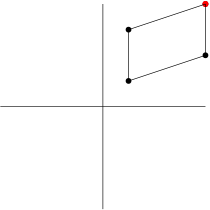
\includegraphics[width=2in]{hw/figs/hw01/q11_9_44.png}
          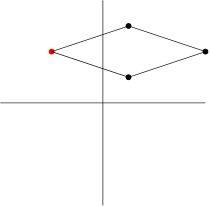
\includegraphics[width=2in]{hw/figs/hw01/q11_9_-22.png}
          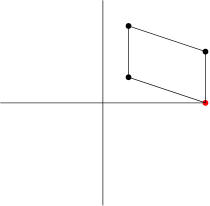
\includegraphics[width=2in]{hw/figs/hw01/q11_9_40.png}
          \caption{Parallelogram points (4,4), (-2,2), and (4,0)}
          \label{fig:09Parallelogram}
        \end{figure}
        
        \item [16.] \textbf{Q.} Mark the point $-\overline{v} + 2\overline{w}$ and any other combination $c\overline{v} + d\overline{w}$ with $c+d = 1$. Draw the line of all combinations that have $c+d=1$. \textbf{A}. Figure \ref{fig:q11_15}.
        
        \begin{figure}
          \centering
          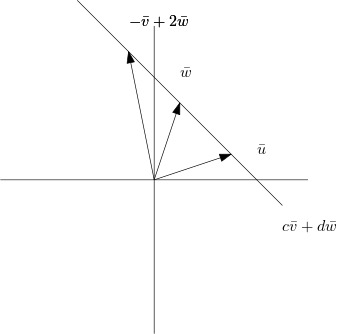
\includegraphics[width=3in]{hw/figs/hw01/q11_15.png}
          \caption{Line of all combinations that have $c+d=1$}
          \label{fig:q11_15}
        \end{figure}
        
        \item [25.] \textbf{Q.} Draw vectors $\bm{u}$, $\bm{v}$, $\bm{w}$ so that their combinations $c\bm{u}+d\bm{v}+e\bm{w}$ fill only a line. Find vectors $\bm{u}$, $\bm{v}$, $\bm{w}$ so that their combinations $c\bm{u}+d\bm{v}+e\bm{w}$ fill only a plane. \textbf{A.} Figure \ref{fig:s11_q25}.
        
        \begin{figure}
          \centering
          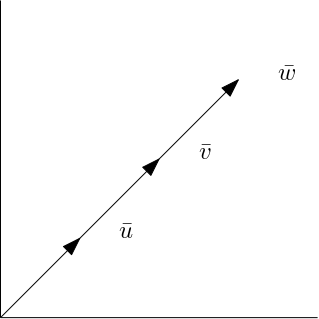
\includegraphics[width=2in]{hw/figs/hw01/s11_q25_line.png}
          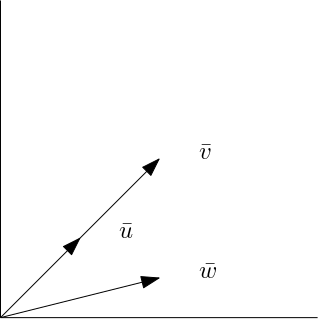
\includegraphics[width=2in]{hw/figs/hw01/s11_q25_plane.png}
          \caption{Line and plane}
          \label{fig:s11_q25}
        \end{figure}
        
    \end{enumerate}

\subsection{Section 1.2}

    \begin{enumerate}
        \item [3.] \textbf{Q.} Find unit vectors in the direction of $ \bm{v} = \left[\begin{array}{l} 3 \\ 4\end{array}\right]$ and $\bm{w} = \left[\begin{array}{l}8 \\ 6\end{array}\right]$ and the cosine for the angle $\theta$. Choose vectors $\bm{a}$, $\bm{b}$, and $\bm{c}$ that make $0^{\circ}, 90^{\circ}$ and $180^{\circ}$ angles with $\bm{w}$. \textbf{A}.
        
        $$
        \begin{aligned}
            \frac{\bm{v}}{\|\bm{v}\|} & = \frac{\bm{v}}{\sqrt{3^2 + 4^2}} = \left[\begin{array}{l} 3/5 \\ 4/5 \end{array}\right]\\
            \frac{\bm{w}}{\|\bm{w}\|} & = \frac{\bm{w}}{\sqrt{8^2 + 6^2}} = \left[\begin{array}{l} 4/5 \\ 3/5 \end{array}\right]\\
            \cos(\theta) & = \frac{\bm{v}\cdot\bm{w}}{\|\bm{v}\|\|\bm{w}\|} 
            = \frac{24}{25}\\
            \bm{u} & = \left[\begin{array}{l} -.6 \\ .8\end{array}\right] \\
            \frac{\bm{w}\cdot\bm{w}}{\|\bm{w}\|\|\bm{w}\|} & = \frac{-4.8 + 4.8}{\|\bm{u}\|\|\bm{w}\|} = 0 = \cos(0)\\
            \frac{\bm{u}\cdot\bm{w}}{\|\bm{u}\|\|\bm{w}\|} & = \frac{-4.8 + 4.8}{\|\bm{u}\|\|\bm{w}\|} = 0 = \cos(90)\\
        \end{aligned}
        $$
        
        \item [11.] \textbf{Q.} If $\bm{v} \cdot \bm{w}$ is negative, what does this say about the angle between $\bm{v}$ and $\bm{w}$? Draw a 3-dimensional vector $\bm{v}$ (an arrow), and show where to find all $\bm{w}$'s with $\bm{v} \cdot \bm{w} < 0$. \textbf{A.}
        
        $$
        \bm{v} \cdot \bm{w}=\|v\|\|w\| \cos \theta
        $$
        
        The magnitude of the vector is always positive so a negative dot product indicates that $\cos\theta$ is negative $\therefore \theta > 90^{\circ}$. Reference Figure \ref{fig:s12_q11}.
        
        \begin{figure}
          \centering
          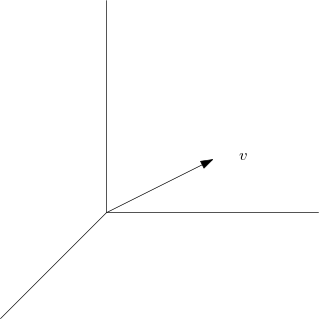
\includegraphics[width=2in]{hw/figs/hw01/s12_q11.png}
          \caption{The angle $\theta$ must be greater than $90^{\circ}$ between $\bm{v}$ and $\bm{w}$ with the set of $\bm{w}$ vectors filling half the three dimensional space.}
          \label{fig:s12_q11}
        \end{figure}
        
        \item [17.] \textbf{Q.} What are the cosines of the angles $\alpha$, $\beta$, $\theta$ between the vector (1,0,-1) and the unit vectors $\bm{i}$, $\bm{j}$, and $\bm{k}$ along the axes? Check the formula $\cos^2 \alpha + \cos^2 \beta + \cos^2 \theta = 1$. \textbf{A.}
        
        $$
        \begin{aligned}
            \bm{v} \bm{w}                   & =\|v\|\|w\| \cos \theta \\
             v_1 w_1 + v_2 w_2 + v_3 w_3    & =\|v\|\|w\| \cos \theta \\
             (1)(1) + (0)(0) + (-1)(0)      & = \sqrt{1^2 + 0^2 + -1^2} \sqrt{1^2 + 0^2 + 0^2} \cos \alpha \\
             1                              & = \sqrt{2} \cos(\alpha) \\
             \cos(\alpha)                   & = \frac{1}{\sqrt{2}} \\  
             (1)(0) + (0)(1) + (-1)(0)      & = \sqrt{1^2 + 0^2 + -1^2} \sqrt{0^2 + 1^2 + 0^2} \cos \alpha \\
             0                              & = \sqrt{2} \cos(\alpha) \\
             \cos(\beta)                    & = 0 \\ 
             (1)(0) + (0)(0) + (-1)(1)      & = \sqrt{1^2 + 0^2 + -1^2} \sqrt{0^2 + 0^2 + 1^2} \cos \alpha \\
             -1                             & = \sqrt{2} \cos(\alpha) \\
             \cos(\theta)                   & = -\frac{1}{\sqrt{2}} \\ 
        \end{aligned}
        $$
        
        \item [21.] \textbf{Q.} The triangle inequality says: $(\text{length of } \bm{v} + \bm{w}) \leq ( \text{length of } \bm{v} ) + ( \text{length of } \bm{w} )$. Problem 19 found $\| \bm{v} + \bm{w} \|^2 = \|v\|^2 + 2 \bm{v} \cdot \bm{w} + \|w\|^2$. Use the Schwarz inequality $\bm{v} \cdot \bm{w} \leq \|v\| \|w\|$ to show that $\|\textbf{side 3}\|$ can not exceed $\|\textbf{side 1}\| + \|\textbf{side 2}\|$: 
        
        $$\text{Triangle inequality: }\|v+w\|^{2} \leq(\|v\|+\|w\|)^{2} \quad \text{ or } \quad\|v+w\| \leq\|v\|+\|w\|$$ 
        
        \textbf{A.}
        
        
        \begin{align*}
            \|v+w\|^{2} & = \|v\|^{2}+2 v \cdot w+\|w\|^{2} \\
            \|v+w\|^{2} & \leq \|v\|^{2}+2 \|v\|\|w\| +\|w\|^{2} \tag{by Schwarz inequality} \\
            \|v+w\|^{2} & \leq(\|v\|+\|w\|)^{2} \tag{by formula $a^{2}+2 a b+b^{2}=(a+b)^{2}$}
        \end{align*}
        
        \item [29.] \textbf{Q.} Pick any numbers that add to $x+y+z=0$. Find the angle between your vector $\bm{v}=(x, y, z)$ and the vector $\bm{w}=(z, x, y)$. Challenge question: Explain why $\bm{v} \cdot \bm{w} /\|\bm{v}\|\|\bm{w}\|$ is always $-\frac{1}{2}$. \textbf{A.} 
        
        \begin{align*}
            \bm{v} & = (1, 4, -5) \\
            \bm{w} & = (-5, 1, 4) \\
            \cos \theta & = \frac{\bm{v} \cdot \bm{w}}{\|\bm{v}\|\|\bm{w}\|} \\
                        & = \frac{(1 \times-5)+(4 \times 1)+(-5 \times 4)}
                        {\sqrt{1^{2}+4^{2}+(-5)^{2}} \cdot \sqrt{(-5)^{2}+(1)^{2}+(4)^{2}}}\\
                        & = \frac{-21}{42} \\
                        & = \frac{-1}{2}
        \end{align*}
        
        Challenge question
        
        \begin{align*}
            \bm{v} \cdot \bm{w} & = x z + y z + x y \\
                                & =\frac{1}{2}(x+y+z)^{2}-\frac{1}{2}\left(x^{2}+y^{2}+z^{2}\right) \\
        \end{align*}
        
    \end{enumerate}

\subsection{Section 1.3}

    \begin{enumerate}
        \item [1.] \textbf{Q.} Find the linear combination $2 \bm{s}_{1}+3 \bm{s}_{2}+4 \bm{s}_{3}=\bm{b}$. Then write $\bm{b}$ as a matrix-vector multiplication $S \bm{x}$. Compute the dot products (row of $S$ ) $\cdot \bm{x}$ :
        
        $$
        \bm{s}_{1}=\left[\begin{array}{l}
        1 \\
        1 \\
        1
        \end{array}\right] \quad \bm{s}_{2}=\left[\begin{array}{l}
        0 \\
        1 \\
        1
        \end{array}\right] \quad \bm{s}_{3}=\left[\begin{array}{l}
        0 \\
        0 \\
        1
        \end{array}\right] \text { go into the columns of } S.
        $$
        
        \textbf{A.}
        
        linear combination
        
        $$
        \begin{aligned}
        \boldsymbol{b} &=2 \boldsymbol{s}_{1}+3 \boldsymbol{s}_{2}+4 \boldsymbol{s}_{3} \\
        &=2\left[\begin{array}{l}
        1 \\
        1 \\
        1
        \end{array}\right]+3\left[\begin{array}{l}
        0 \\
        1 \\
        1
        \end{array}\right]+4\left[\begin{array}{l}
        0 \\
        0 \\
        1
        \end{array}\right] \\
        &=\left[\begin{array}{l}
        2 \\
        2 \\
        2
        \end{array}\right]+\left[\begin{array}{l}
        0 \\
        3 \\
        3
        \end{array}\right]+\left[\begin{array}{l}
        0 \\
        0 \\
        4
        \end{array}\right] \\
        &=\left[\begin{array}{l}
        2+0+0 \\
        2+3+0 \\
        2+3+4
        \end{array}\right] \\
        &=\left[\begin{array}{l}
        2 \\
        5 \\
        9
        \end{array}\right]
        \end{aligned}
        $$
        
        matrix-vector multiplication
        
        $$
        \bm{b}=\left[\begin{array}{lll}
        1 & 0 & 0 \\
        1 & 1 & 0 \\
        1 & 1 & 1
        \end{array}\right]\left[\begin{array}{l}
        2 \\
        3 \\
        4
        \end{array}\right]
        $$
        
        dot product with vector $\bm{x}=(2,3,4)$
        
        $$
        \begin{aligned}
        {\left[\begin{array}{l}
        (1,0,0) \cdot \bm{x} \\
        (1,1,0) \cdot \bm{x} \\
        (1,1,1) \cdot \bm{x}
        \end{array}\right]} & = {\left[\begin{array}{l}
        (1,0,0) \cdot(2,3,4) \\
        (1,1,0) \cdot(2,3,4) \\
        (1,1,1) \cdot(2,3,4)
        \end{array}\right] } \\
        &=\left[\begin{array}{l}
        (1)(2)+(0)(3)+(0)(4) \\
        (1)(2)+(1)(3)+(0)(4) \\
        (1)(2)+(1)(3)+(1)(4)
        \end{array}\right] \\
        & =\left[\begin{array}{l}
        2+0+0 \\
        2+3+0 \\
        2+3+4
        \end{array}\right] \\
        & =\left[\begin{array}{l}
        2 \\
        5 \\
        9
        \end{array}\right]
        \end{aligned}
        $$
        
        \item [2.] \textbf{Q.} Solve these equations $S \bm{y}=\bm{b}$ with $\bm{s}_{1}, \bm{s}_{2}, \bm{s}_{3}$ in the columns of $S:$
        
        $$
        \left[\begin{array}{lll}
        1 & 0 & 0 \\
        1 & 1 & 0 \\
        1 & 1 & 1
        \end{array}\right]\left[\begin{array}{l}
        y_{1} \\
        y_{2} \\
        y_{3}
        \end{array}\right]=\left[\begin{array}{l}
        1 \\
        1 \\
        1
        \end{array}\right] \text { and }\left[\begin{array}{lll}
        1 & 0 & 0 \\
        1 & 1 & 0 \\
        1 & 1 & 1
        \end{array}\right]\left[\begin{array}{l}
        y_{1} \\
        y_{2} \\
        y_{3}
        \end{array}\right]=\left[\begin{array}{l}
        1 \\
        4 \\
        9
        \end{array}\right] \text {. }
        $$
        What is the sum of the first $n$ odd numbers? \textbf{A.}
        
        First equation
        
        $$
        \begin{aligned}
        \left[\begin{array}{l}
        y_{1}(1)+y_{2}(0)+y_{3}(0) \\
        y_{1}(1)+y_{2}(1)+y_{3}(0) \\
        y_{1}(1)+y_{2}(1)+y_{3}(1)
        \end{array}\right] & = \left[\begin{array}{l}
        1 \\
        1 \\
        1
        \end{array}\right]\\
        y_{1} & =1 \\
        y_{1}+y_{2} & = 1 \\
        y_{1}+y_{2}+y_{3} & = 1 \\
        y_{1} & = 1 \\
        y_{2} & = 0 \\
        y_{3} & = 0
        \end{aligned}
        $$
        
        Second Equation

        $$
        \begin{aligned}
        \left[\begin{array}{l}
        y_{1}(1)+y_{2}(0)+y_{3}(0) \\
        y_{1}(1)+y_{2}(1)+y_{3}(0) \\
        y_{1}(1)+y_{2}(1)+y_{3}(1)
        \end{array}\right] & =\left[\begin{array}{l}
        1 \\
        4 \\
        9
        \end{array}\right] \\
        y_{1} & =1 \\
        y_{1}+y_{2} & =4 \\
        y_{1}+y_{2}+y_{3} & = 9 \\
        y_{1} & = 1 \\
        y_{2} & = 3 \\
        y_{3} & = 5 \\
        \end{aligned}
        $$
        
        The sum of the first $n$ odd numbers is $n^2$.
        
        \item [4.] \textbf{Q.} Find a combination $x_{1} \bm{w}_{1} + x_{2} \bm{w}_{2} + x_{3} \bm{w}_{3}$ that gives the zero vector:
        
        $$
        \bm{w}_{1}=\left[\begin{array}{l}
        1 \\
        2 \\
        3
        \end{array}\right] \quad \bm{w}_{2}=\left[\begin{array}{l}
        4 \\
        5 \\
        6
        \end{array}\right] \quad \bm{w}_{3}=\left[\begin{array}{l}
        7 \\
        8 \\
        9
        \end{array}\right]
        $$
        
        Those vectors are (independent) (dependent)? What do the three vectors lie in? The matrix $W$ with those columns is not invertible. \textbf{A.}
        
        $$
        \begin{aligned}
        \left[\begin{array}{l}
        x_{1}+4 x_{2}+7 x_{3} \\
        2 x_{1}+5 x_{2}+8 x_{3} \\
        3 x_{1}+6 x_{2}+9 x_{3}
        \end{array}\right] & =\left[\begin{array}{l}
        0 \\
        0 \\
        0
        \end{array}\right] \\
        2R_1 - R_2 \rightarrow 3x_2 + 6x_3 & = 0 \\
        x_2 & = -2x_3 \\
        6R_2 - 5R_3 \rightarrow -3x_1 + 3x_3 & = 0 \\
        x_1 & = x_3
        \end{aligned}
        $$
        
        $\frac{x_{1}}{1}=\frac{x_{2}}{-2}=\frac{x_{3}}{1} \therefore$ a non-zero solution to the system of equations is $x_{1}=1, x_{2}=-2, x_{3}=1$. The above sum needs to be a zero vector, so the vectors are dependent, and they lie in a plane.
        
        \item [7.] \textbf{Q.} If the columns combine into $A \bm{x}=\bm{0}$ then each row has $\bm{r} \cdot \bm{x}=0$ :
        
        $$
        \left[\begin{array}{lll}
        \bm{a}_{1} & \bm{a}_{2} & \bm{a}_{3}
        \end{array}\right]\left[\begin{array}{l}
        x_{1} \\
        x_{2} \\
        x_{3}
        \end{array}\right]=\left[\begin{array}{l}
        0 \\
        0 \\
        0
        \end{array}\right] \quad \text { By rows }\left[\begin{array}{l}
        \boldsymbol{r}_{1} \cdot \boldsymbol{x} \\
        \boldsymbol{r}_{2} \cdot \boldsymbol{x} \\
        \boldsymbol{r}_{3} \cdot \boldsymbol{x}
        \end{array}\right]=\left[\begin{array}{l}
        0 \\
        0 \\
        0
        \end{array}\right] .
        $$
        
        The three rows also lie in a plane. Why is that plane perpendicular to $\bm{x}$? \textbf{A.} The dot product of any two perpendicular vectors is zero, therefore vectors $\bm{r}_1, \bm{r}_2, \bm{r}_3$ are perpendicular to vector $\bm{x}$. All three rows line in a plane, therefore the plane is perpendicular to $\bm{x}$.
        
    \end{enumerate}

\subsection{Section 2.1}

    \begin{enumerate}
        \item [1.] \textbf{Q.} With $A=I$ (the identity matrix) draw the planes in the row picture. Three sides of a box meet at the solution $\bm{x}=(x, y, z)=(2,3,4)$ :
        
        $$
        \begin{aligned}
        &1 x+0 y+0 z=2 \\
        &0 x+1 y+0 z=3 \\
        &0 x+0 y+1 z=4
        \end{aligned} \quad \text { or } \quad\left[\begin{array}{lll}
        1 & 0 & 0 \\
        0 & 1 & 0 \\
        0 & 0 & 1
        \end{array}\right]\left[\begin{array}{l}
        x \\
        y \\
        z
        \end{array}\right]=\left[\begin{array}{l}
        2 \\
        3 \\
        4
        \end{array}\right] \text {. }
        $$
        
        Draw the vectors in the column picture. Two times column 1 plus three times column 2 plus four times column 3 equals the right side $\bm{b}$. \textbf{A.} Reference Figure \ref{fig:s21_q01}.
        
        \begin{figure}
          \centering
          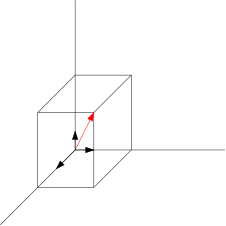
\includegraphics[width=2in]{hw/figs/hw01/s21_q01.png}
          \caption{Red vector $\bm{b}=\left[\begin{array}{l}2 \\ 3 \\ 4\end{array}\right]$ composed of multiples of three unit vectors.}
          \label{fig:s21_q01}
        \end{figure}
        
        
        \item [16.] 
        \begin{enumerate}
            \item [a.] \textbf{Q.}  What 2 by 2 matrix $R$ rotates every vector by $90^{\circ}$ ? $R$ times $\left[\begin{array}{l}\mathbf{x} \\ \mathbf{y}\end{array}\right]$ is $\left[\begin{array}{r}\mathbf{y} \\ -\mathbf{x}\end{array}\right]$. \textbf{A.}
            
            $$R=\left[\begin{array}{cc}0 & 1 \\ -1 & 0\end{array}\right]$$
            
            \item [b.] \textbf{Q.} What 2 by 2 matrix $R^{2}$ rotates every vector by $180^{\circ}$ ? \textbf{A.}
            
            $$
            \begin{aligned}
            R^{2} & =\left[\begin{array}{cc}
            0 & 1 \\
            -1 & 0
            \end{array}\right]\left[\begin{array}{cc}
            0 & 1 \\
            -1 & 0
            \end{array}\right] \\
            R^{2} & = \left[\begin{array}{cc}
            -1 & 0 \\
            0 & -1
            \end{array}\right]
            \end{aligned}
            $$
            
        \end{enumerate} 

        \item [21.] \textbf{Q.} What 2 by 2 matrix $R$ rotates every vector through $45^{\circ}$ ? The vector $(1,0)$ goes to $(\sqrt{2} / 2, \sqrt{2} / 2)$. The vector $(0,1)$ goes to $(-\sqrt{2} / 2, \sqrt{2} / 2)$. Those determine the matrix. Draw these particular vectors in the $x y$ plane and find $R$. \textbf{A.}
        
        $$
        \begin{aligned}
        \operatorname{Rot}_{45^{\circ}}\left(\left[\begin{array}{l}
        1 \\
        0
        \end{array}\right]\right) 
        & =\left[\begin{array}{l}
        \cos 45^{\circ} \\
        \sin 45^{\circ}
        \end{array}\right]
        =\left[\begin{array}{c}
        \frac{1}{\sqrt{2}} \\
        \frac{1}{\sqrt{2}}
        \end{array}\right]
        = \left[\begin{array}{c}
        \frac{\sqrt{2}}{2} \\
        \frac{\sqrt{2}}{2}
        \end{array}\right] \\
        \operatorname{Rot}_{45^{\circ}}\left(\left[\begin{array}{l}
        0 \\
        1
        \end{array}\right]\right)
        & =\left[\begin{array}{c}
        -\sin 45^{\circ} \\
        \cos 45^{\circ}
        \end{array}\right] 
        =\left[\begin{array}{c}
        -\frac{1}{\sqrt{2}} \\
        \frac{1}{\sqrt{2}}
        \end{array}\right]=\left[\begin{array}{c}
        -\frac{\sqrt{2}}{2} \\
        \frac{\sqrt{2}}{2}
        \end{array}\right] \\
        R & = \left[\operatorname{Rot}_{45^{\prime}}\left(\left[\begin{array}{l}
        1 \\
        0
        \end{array}\right]\right) \quad \operatorname{Rot}_{45^{\circ}}\left(\left[\begin{array}{l}
        0 \\
        1
        \end{array}\right]\right)\right]
        = \left[\begin{array}{ll}
        \frac{\sqrt{2}}{2} & -\frac{\sqrt{2}}{2} \\
        \frac{\sqrt{2}}{2} & \frac{\sqrt{2}}{2}
        \end{array}\right]
        \end{aligned}
        $$
        
        Reference Figure \ref{fig:s21_q21}.
        
        \begin{figure}
          \centering
          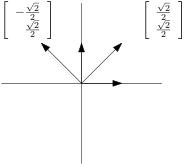
\includegraphics[width=2in]{hw/figs/hw01/s21_q21.png}
          \caption{$R$ vectors}
          \label{fig:s21_q21}
        \end{figure}
        
        \item [29.] \textbf{Q.} Start with the vector $\bm{u}_{0}=(1,0)$. Multiply again and again by the same "Markov matrix" $A=[.8 .3 ; .2 .7]$. The next three vectors are $\boldsymbol{u}_{1}, \boldsymbol{u}_{2}, \boldsymbol{u}_{3}$ :
        
        $$
        \boldsymbol{u}_{1}=\left[\begin{array}{ll}
        .8 & .3 \\
        .2 & .7
        \end{array}\right]\left[\begin{array}{l}
        1 \\
        0
        \end{array}\right]=\left[\begin{array}{l}
        .8 \\
        .2
        \end{array}\right] \quad \boldsymbol{u}_{2}=A \boldsymbol{u}_{1}=? \quad \boldsymbol{u}_{3}=A \boldsymbol{u}_{2}=?
        $$
        
        What property do you notice for all four vectors $\boldsymbol{u}_{0}, \boldsymbol{u}_{1}, \boldsymbol{u}_{2}, \boldsymbol{u}_{3}$ ? \textbf{A.}
        
        $$
        \begin{aligned}
        \bm{u}_2 & = A \bm{u}_1 
        = \left[\begin{array}{ll}
        .8 & .3 \\
        .2 & .7
        \end{array}\right]\left[\begin{array}{l}
        .8 \\
        .2
        \end{array}\right]
        = \left[\begin{array}{l}
        .7 \\
        .3
        \end{array}\right] \\
        \bm{u}_3 & = A\bm{u}_2
        =\left[\begin{array}{ll}
        .8 & .3 \\
        .2 & .7
        \end{array}\right]\left[\begin{array}{l}
        .7 \\
        .3
        \end{array}\right]
        = \left[\begin{array}{l}
        .65 \\
        .35
        \end{array}\right]
        \end{aligned}
        $$
        
        In each vector all components add to 1.
        
        \item [30.] \textbf{Q.} Continue Problem 29 from $u_{0}=(1,0)$ to $\boldsymbol{u}_{7}$, and also from $\boldsymbol{v}_{0}=(0,1)$ to $\boldsymbol{v}_{7}$. What do you notice about $\boldsymbol{u}_{7}$ and $\boldsymbol{v}_{7}$ ? Here are two MATLAB codes, with while and for. They plot $\boldsymbol{u}_{0}$ to $\boldsymbol{u}_{7}$ and $\boldsymbol{v}_{0}$ to $\boldsymbol{v}_{7}$. You can use other languages:
        
        \begin{lstlisting}
        u=[1;0]; A = [.8.3;.2.7];
        x = u; k = [0:7];
        while size (x,2) <= 7
            u = A * u; x=[x u];
        end
        plot(k, x)
        \end{lstlisting}
        
        and
        
        \begin{lstlisting}
        u=[0;1]; A = [.8.3;.2.7];
        x = v; k = [0:7];
        for j = 1 : 7
            v = A * u; x=[x v];
        end
        plot(k, x)
        \end{lstlisting}
        
        The $\boldsymbol{u}$ 's and $\boldsymbol{v}$ 's are approaching a steady state vector $\boldsymbol{s}$. Guess that vector and check that $A \bm{s}=\bm{s}$. If you start with $\bm{s}$, you stay with $\bm{s}$. \textbf{A.}
        
        The steady state vector 
        
        $$
        \left[\begin{array}{ll}
        .8 & .3 \\
        .2 & .7
        \end{array}\right]\left[\begin{array}{l}
        .6 \\
        .4
        \end{array}\right]=\left[\begin{array}{l}
        .6 \\
        .4
        \end{array}\right]
        $$
        
        There is no change when multiplied by $\left[\begin{array}{rr}.8 & .3 \\ .2 & .7\end{array}\right]$.
        
    \end{enumerate}

\subsection{Section 2.3}

    \begin{enumerate}
        \item [1.] \textbf{Q.} Write down the 3 by 3 matrices that produce these elimination steps:
        \begin{enumerate}
            \item [a.] $E_{21}$ subtracts 5 times row 1 from row 2 .
            \item [b.] $E_{32}$ subtracts $-7$ times row 2 from row 3 .
            \item [c.] $P$ exchanges rows 1 and 2 , then rows 2 and 3 .
        \end{enumerate}
        \textbf{A.}
        
        $$
        \begin{aligned}
        I & =\left[\begin{array}{lll}
        1 & 0 & 0 \\
        0 & 1 & 0 \\
        0 & 0 & 1
        \end{array}\right] \\
        E_{21} & = \left[\begin{array}{ccc}
        1 & 0 & 0 \\
        -5 & 1 & 0 \\
        0 & 0 & 1
        \end{array}\right] \\
        E_{32} & =\left[\begin{array}{lll}
        1 & 0 & 0 \\
        0 & 1 & 0 \\
        0 & 7 & 1
        \end{array}\right] \\
        P_{12} & =\left[\begin{array}{lll}
        0 & 1 & 0 \\
        1 & 0 & 0 \\
        0 & 0 & 1
        \end{array}\right] \\
        P_{23} & =\left[\begin{array}{lll}
        1 & 0 & 0 \\
        0 & 0 & 1 \\
        0 & 1 & 0
        \end{array}\right] \\
        P = P_{23} P_{12} & = 
        \left[\begin{array}{lll}
        0 & 1 & 0 \\
        0 & 0 & 1 \\
        1 & 0 & 0
        \end{array}\right]
        \end{aligned}
        $$

        \item [7a.] \textbf{Q. (Only part a)} Suppose $E$ subtracts 7 times row 1 from row 3 .
            \begin{enumerate}
                \item [a.] To invert that step you should $\ldots$ 7 times row $\ldots$ to row $\ldots$
            \end{enumerate}
            \textbf{A.}
            
            $$
            \begin{aligned}
            E & =\left[\begin{array}{ccc}
            1 & 0 & 0 \\
            0 & 1 & 0 \\
            -7 & 0 & 1
            \end{array}\right] \\
            E E^{-1} & = I \\
            E^{-1} & =\left[\begin{array}{lll}
            1 & 0 & 0 \\
            0 & 1 & 0 \\
            7 & 0 & 1
            \end{array}\right] \\
            E^{-1} E & = I \\
            \end{aligned}
            $$
            
        \item [9.] 
        \begin{enumerate}
            \item [a.] \textbf{Q.}  $E_{21}$ subtracts row 1 from row 2 and then $P_{23}$ exchanges rows 2 and 3. What matrix $M=P_{23} E_{21}$ does both steps at once? \textbf{A.}
            
            $$
            \begin{aligned}
            E_{21} & = \left[\begin{array}{ccc}
            1 & 0 & 0 \\
            -1 & 1 & 0 \\
            0 & 0 & 1
            \end{array}\right] \\
            P_{23} & = \left[\begin{array}{lll}
            1 & 0 & 0 \\
            0 & 0 & 1 \\
            0 & 1 & 0
            \end{array}\right] \\
            M & =P_{23} E_{21} \\
            & =\left[\begin{array}{lll}
            1 & 0 & 0 \\
            0 & 0 & 1 \\
            0 & 1 & 0
            \end{array}\right]\left[\begin{array}{ccc}
            1 & 0 & 0 \\
            -1 & 1 & 0 \\
            0 & 0 & 1
            \end{array}\right] \\
            & =\left[\begin{array}{ccc}
            1 & 0 & 0 \\
            0 & 0 & 1 \\
            -1 & 1 & 0
            \end{array}\right]
            \end{aligned}
            $$
            
            \item [b.] \textbf{Q.}  $P_{23}$ exchanges rows 2 and 3 and then $E_{31}$ subtracts row 1 from row 3 . What matrix $M=E_{31} P_{23}$ does both steps at once? Explain why the $M$'s are the same but the $E$ 's are different. \textbf{A.}
            
            $$
            \begin{aligned}
            E_{31} & = \left[\begin{array}{ccc}
            1 & 0 & 0 \\
            0 & 1 & 0 \\
            -1 & 0 & 1
            \end{array}\right] \\
            P_{23} & = \left[\begin{array}{ccc}
            1 & 0 & 0 \\
            0 & 0 & 1 \\
            0 & 1 & 0
            \end{array}\right] \\
            M & =E_{31} P_{23} \\
            & =\left[\begin{array}{ccc}
            1 & 0 & 0 \\
            0 & 1 & 0 \\
            -1 & 0 & 1
            \end{array}\right]\left[\begin{array}{lll}
            1 & 0 & 0 \\
            0 & 0 & 1 \\
            0 & 1 & 0
            \end{array}\right] \\
            & =\left[\begin{array}{ccc}
            1 & 0 & 0 \\
            0 & 0 & 1 \\
            -1 & 1 & 0
            \end{array}\right]
            \end{aligned}
            $$
            
            In a. we subtract row 1 from row 2 then exchange it so that eliminated row is row 3, while in b. we first exchange row 2 and 3 then subtract row 1 from row 3 so that the eliminated row is row 3.
            
        \end{enumerate}
        
        \item [12.] \textbf{Q.} Multiply these matrices:
            $$
            \left[\begin{array}{lll}
            0 & 0 & 1 \\
            0 & 1 & 0 \\
            1 & 0 & 0
            \end{array}\right]\left[\begin{array}{lll}
            1 & 2 & 3 \\
            4 & 5 & 6 \\
            7 & 8 & 9
            \end{array}\right]\left[\begin{array}{lll}
            0 & 0 & 1 \\
            0 & 1 & 0 \\
            1 & 0 & 0
            \end{array}\right] \quad\left[\begin{array}{rrr}
            1 & 0 & 0 \\
            -1 & 1 & 0 \\
            -1 & 0 & 1
            \end{array}\right]\left[\begin{array}{lll}
            1 & 2 & 3 \\
            1 & 3 & 1 \\
            1 & 4 & 0
            \end{array}\right] \text {. }
            $$
            \textbf{A.}
            
            $$
            \begin{aligned}
            \left[\begin{array}{lll}
            0 & 0 & 1 \\
            0 & 1 & 0 \\
            1 & 0 & 0
            \end{array}\right]\left[\begin{array}{lll}
            1 & 2 & 3 \\
            4 & 5 & 6 \\
            7 & 8 & 9
            \end{array}\right] & = \left[\begin{array}{lll}
            7 & 8 & 9 \\
            4 & 5 & 6 \\
            1 & 2 & 3
            \end{array}\right] \\
            \left[\begin{array}{lll}
            7 & 8 & 9 \\
            4 & 5 & 6 \\
            1 & 2 & 3
            \end{array}\right]\left[\begin{array}{lll}
            0 & 0 & 1 \\
            0 & 1 & 0 \\
            1 & 0 & 0
            \end{array}\right] & = \left[\begin{array}{lll}
            9 & 8 & 7 \\
            6 & 5 & 4 \\
            3 & 2 & 1
            \end{array}\right] \\
            \left[\begin{array}{ccc}
            1 & 0 & 0 \\
            -1 & 1 & 0 \\
            -1 & 0 & 1
            \end{array}\right]\left[\begin{array}{lll}
            1 & 2 & 3 \\
            1 & 3 & 1 \\
            1 & 4 & 0
            \end{array}\right] & =\left[\begin{array}{ccc}
            1 & 2 & 3 \\
            0 & 1 & -2 \\
            0 & 2 & -3
            \end{array}\right]
            \end{aligned}
            $$
        
        \item [22.]  The entries of $A$ and $\bm{x}$ are $a_{i j}$ and $x_{j}$. So the first component of $A \bm{x}$ is $\sum a_{1 j} x_{j}=$ $a_{11} x_{1}+\cdots+a_{1 n} x_{n}$. If $E_{21}$ subtracts row 1 from row 2 , write a formula for
        \begin{enumerate}
            \item [a.] \textbf{Q.} the third component of $A \bm{x}$. 
            \textbf{A.} $\sum a_{3 j} x_{j}=a_{31} x_{1}+a_{32} x_{2}+\ldots+a_{3 n} x_{n}$
            
            \item [b.] \textbf{Q.} the $(2,1)$ entry of $E_{21} A$. 
            \textbf{A.} $a_{21}-a_{11}$
            
            \item [c.] \textbf{Q.} the $(2,1)$ entry of $E_{21}\left(E_{21} A\right)$. 
            \textbf{A.} $a_{21}-2 a_{11}$
            
            \item [d.] \textbf{Q.} the first component of $E_{21} A \bm{x}$. 
            \textbf{A.} The sum of the product of the elements of the matrix $E_{21} A$ with the corresponding elements of the vector $x$ which is 
            $a_{11} x_{1}+a_{12} x_{2}+\ldots+a_{1 n} x_{n}$.

        \end{enumerate}

    \end{enumerate}

\end{document}